\section{Domain decomposition}
% * <felipe.cruz.v@gmail.com> 2018-06-04T10:33:10.994Z:
% 
% > Domain decomposition
% I think you need a high level explanation before jumping into the details, otherwise you would have to read the whole section to infer what is going on. I.e.:
% Can you explain at the start of this section what is the objective of the domain decomposition from a very abstract point of view (e.g. distribute partitions of the domain among multiple compute nodes)? and how it achieves the goal with pseudo code:
% * what are the inputs
% * how that inputs if transformed into subdivision
% * how the models for the compute and communication for each cell is built
% *how the optimization is run to load balance
% * what is the output
% 
% ^.
Domain decomposition in the context of this thesis refers to the process of dividing a computational domain into smaller parts in order to run on multiple processing units.
Specifically, domain decomposition here is not be confused with the \textit{domain decomposition method} in mathematics and numerical analysis which is used to solve boundary value problems by splitting them into smaller parts.
Instead, domain decomposition in high performance computing and this thesis is the name of a process used for solving partial differential equations using finite difference methods on multiple processing units.

The next sections outline the general approach to domain decomposition and afterwards the specifics of the model developed and used in this thesis.

\subsection{General approach}



%As mentioned in the introduction (sec. \ref{sec:intro_source_graph}) domain decomposition using graph partitioning algorithms requires a source graph.
%For finite element codes the source graph is usually the same as the mesh file describing the physical domain infused with additional information about communication costs.
%However, for finite difference codes running on regular grids with large amount of grid elements this would be an impractically large source graph.
%Instead the following section will describe a model to be used to simplify the source graph generation process.
\subsection{Subdivision model for source graph generation}
As mentioned before source graphs where every source graph node represents a single physical domain grid point would be impractical for large domains.
Therefore, any alternative has to combine some of these domain grid points into separate divisions even before the domain decomposition occurs.

The simplest method of subdividing a regular grid is by splitting it across each dimension separately, i.e. creating a number of uniform subdivisions.

This guarantees that every subdivision has the same amount of neighbors, with the exception of sections at the boundary of the physical domain if the boundary is not periodic.
Also every subdivision has the same size and therefore distributing them equally during the graph partitioning also means distributing the grid points equally.

Also for this kind of subdivisions it is simple to define the interior and boundary between subdivisions.

One limit to the minimal size of a subdivision in any direction is given by the corresponding stencil extend.
Meaning a stencil can not extend into multiple subdivisions, but only the direct neighbor, otherwise subdivision would have multiple neighbors in the same direction.
This should not be a problem, since usually stencils are not as large as any reasonable sized subdivision.

\subsubsection{Communication cost}
The communication cost between subdivisions is the main criteria being minimized in the graph partitioning algorithm.
Splitting the domain into uniform subdivisions keeps the communication cost computation simple.

The communication cost for each neighbor of the subdivision is determined by the size of the boundary between the two and the extent of the stencil in the corresponding direction.

For three dimensional domains the communication cost can therefore be computed from the following formula:
\begin{equation}
cc\left(i\right) = sds\left(\left(\floor[\Big]{\frac{i}{2}} - 1\right) \% 3 \right) \cdot sds\left(\left(\floor[\Big]{\frac{i}{2}} + 1\right) \% 3 \right) \cdot se\left(i\right)
\end{equation}
where $cc\left(i\right)$ is the communication cost for side $i$.
The index $i \in \left[0, 1, 2, 3, 4, 5\right]$ is combination of side and dimension, i.e. $0$ is negative x direction, $1$ is positive x-direction, $2$ is negative y-direction and so on.
$sds\left(j\right)$ is the subdivision size of dimension $j \in \left[0,1,2]$.
Lastly $se\left(i\right)$ is the stencil extend of side and dimension $i$.
The division, rounding and modulo in the formula is simply a short version of selecting the index of the other two dimensions for the computation of the area between two subdivisions.

\subsubsection{Computational cost}

The computational cost, corresponding also to the vertex weight in the source graph, is even easier to compute, since it is proportional to the number of grid points inside the subdivision.

\subsubsection{Example subdivision and domain decomposition}
The following example should highlight some aspects of the discussed subdivision and domain decomposition.

All the following figures in this section use the same domain and stencil.
The domain has size $2048 \times 1024 \times 40$ and the stencil extends are given as $\left[1, 1, 1, 1, 0, 0\right]$.
This means the stencil uses $1$ neighboring grid point in negative and positive x- and y-direction.
The boundary of the domain is also periodic in x-direction and non-periodic in y- and z- direction.

The figures \ref{fig:metis1}, \ref{fig:pymetis1}, and \ref{fig:scotch1} show the results if the domain is split into $16 \times 8 \times 1$ subdivisions.
This means every box in the figures represents $128 \times 128 \times 40$ grid points.

For comparison the figures \ref{fig:metis2}, \ref{fig:pymetis2}, and \ref{fig:scotch2} show the results if the domain is split into $32 \times 16 \times 1$ subdivisions.
This means every box in the figures represents $32 \times 32 \times 40$ grid points and 4 of these boxes correspond to one box in the figures on the left side.

This comparison should highlight the difference the number of subdivisions and their size can make for the overall domain decomposition.
Also the difference the graph partitioning can make is shown in fig. \ref{fig:rectangular1}.


\begin{figure}[!htbp]
\centering
\begin{subfigure}{0.6\textwidth}
  \centering
  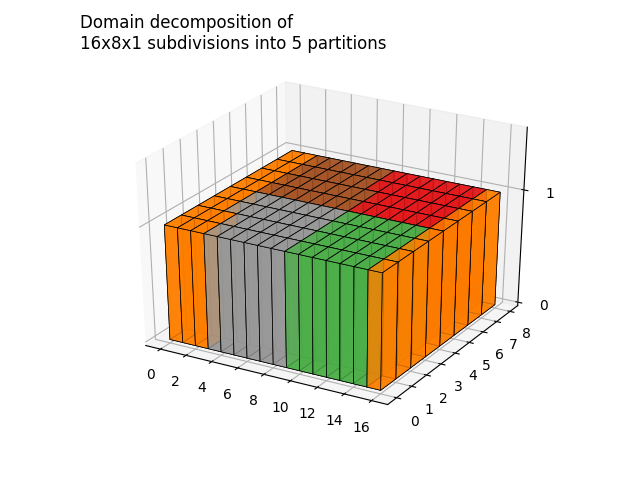
\includegraphics[width=0.9\linewidth]{metis16Px8x1.png}
  \caption{Partitioned by Metis.}
  \label{fig:metis1}
\end{subfigure}%
\begin{subfigure}{0.6\textwidth}
  \centering
  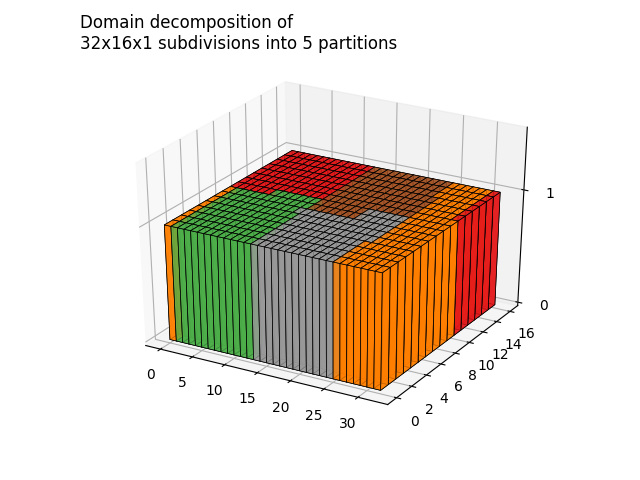
\includegraphics[width=0.9\linewidth]{metis32Px16x1.png}
  \caption{Partitioned by Metis.}
  \label{fig:metis2}
\end{subfigure}

\begin{subfigure}{0.6\textwidth}
  \centering
  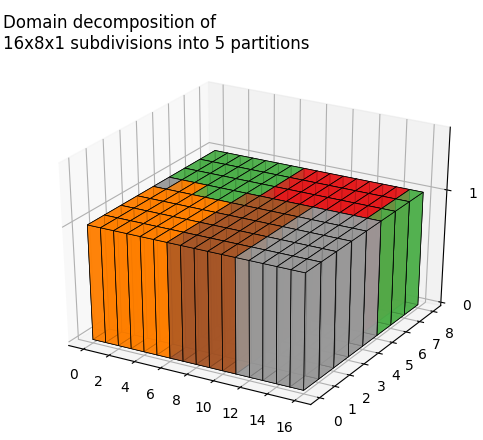
\includegraphics[width=0.9\linewidth]{pymetis16Px8x1.png}
  \caption{Partitioned by PyMetis}
  \label{fig:pymetis1}
\end{subfigure}%
\begin{subfigure}{0.6\textwidth}
  \centering
  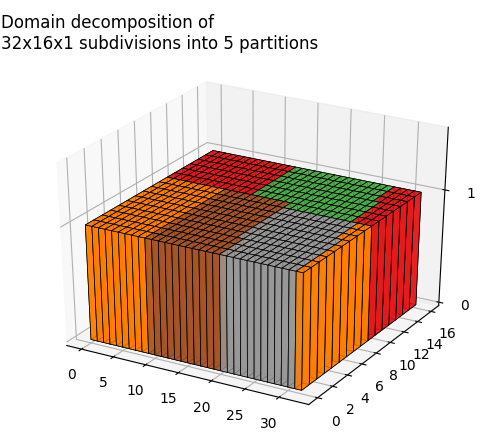
\includegraphics[width=0.9\linewidth]{pymetis32Px16x1.png}
  \caption{Partitioned by PyMetis}
  \label{fig:pymetis2}
\end{subfigure}

\begin{subfigure}{0.6\textwidth}
  \centering
  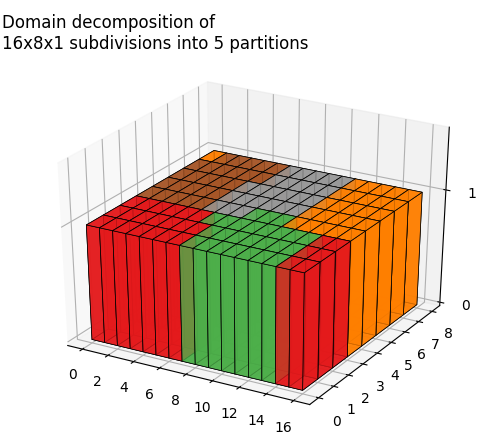
\includegraphics[width=0.9\linewidth]{scotch16Px8x1.png}
  \caption{Partitioned by Scotch}
  \label{fig:scotch1}
\end{subfigure}%
\begin{subfigure}{0.6\textwidth}
  \centering
  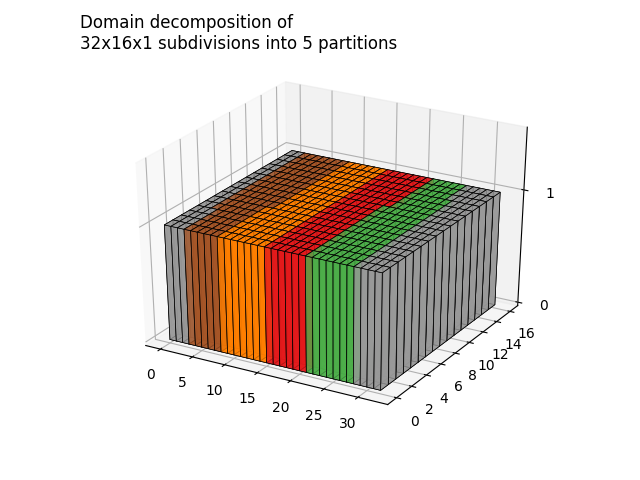
\includegraphics[width=0.9\linewidth]{scotch32Px16x1.png}
  \caption{Partitioned by Scotch}
  \label{fig:scotch2}
\end{subfigure}

\caption{Domain subdivision and domain decomposition into 5 partitions. 
Each box represents one subdivision of grid points.
Each color represents one partition. 
The domain has the size 2048 x 1024 x 40 and a periodic boundary in x-direction.
Even though, the domain is fully three dimensional the domain is only decomposed in the x-y plane i.e. the horizontal plane.
Such a decomposition represents an often encountered use case for domains where the size of the horizontal dimensions are much larger than the size of the vertical dimension e.g. numerical weather prediction models.
Not decomposing in the vertical dimension is important for locality and performance since the vertical dimension is usually the innermost loop dimension.
This also fits with many parameterizations that use the single column model assumption.
}
\label{fig:rectangular1}
\end{figure}

